\section{Evaluation}\label{sec:evaluation}

We evaluate how \textit{effective} interval weakening is in understanding the temporal behaviour of specifications, and how applicable it is to real-world requirements. To this end, we investigate the following research questions:
\begin{itemize}
    \item[\textbf{RQ1:}] To what extent is \cegiw{} useful during the system design phase? (\cref{subsec:demonstration})
    % \marienote{I'm not sure `real-world' is accurate here for the foraging example, maybe try `system design-phase' instead?}
    \item[\textbf{RQ2:}] To what extent can \cegiw{} be used in real-world requirements? (\cref{subsec:case-studies})
    % \marienote{make this more specific: our interval weakening algorithm}
\end{itemize}
%
% \marienote{I feel like there should be some LTL tool citations listed here.}
\textbf{Choosing a model checker.} There are no industrial-strength model checkers for \MTL{} with pointwise semantics~\cite{brihaye2018, akshay2025}, yet many efficient tools exist for linear temporal logic~\cite{cavada2014,holzmann1997} (\LTL{}). Thus, we translate \MTL{} formulae into \LTL{} using the \emph{next} ($X$) operator~\cite[Remark~5.15]{baier2008a} and use an \LTL{} model checker. During preliminary investigation, it was found that symbolic \LTL{} model checkers such as \nuXmv{}~\cite{cavada2014} and \spin{}~\cite{holzmann1997} typically generate minimal counterexample traces. Weakening intervals with these usually only increments or decrements the bound rather than modifying it by a larger amount, which increases the number of calls made to the model checker dramatically. Our implementation\footnote{\url{https://github.com/benmandrew/CEGIW}} uses \nuXmv{} in bounded model checking (BMC) mode, producing multiple counterexamples for a specific bound length, finding the optimal interval for each of them and returning the weakest, making it more likely that we make fewer calls to the model checker. For our implementation we require the user to choose the BMC bound, but theoretical completeness can be preserved as completeness thresholds do exist for BMC~\cite{clarke2004a}.

\subsection{Demonstration of \cegiw{} (RQ1)}\label{subsec:demonstration}

To address \textbf{RQ1}, we use an example based on a model of a foraging robot swarm~\cite{liu2010}. Robots are located in an arena and do a random walk to find food, which they then carry back to their home. Here they recharge and then repeat their foraging task. We model a single robot with a state machine, depicted abstractly in \cref{fig:foraging-fsm}.
%
\begin{figure}[t]
\centering
\begin{tikzpicture}[node distance=1.5cm and 3.5cm, on grid, auto]
\node[state] (deposit) {\texttt{deposit}};
\node[state, above=of deposit] (movetohome) {\texttt{moveToHome}};
\node[state, right=of movetohome] (grabfood) {\texttt{grabFood}};
\node[state, right=of grabfood] (movetofood) {\texttt{moveToFood}};
\node[state, right=of deposit] (homing) {\texttt{homing}};
\node[state, right=of homing] (scanarena) {\texttt{scanArena}};
\node[state, below=of deposit] (resting) {\texttt{resting}};
\node[left=5em of resting] (inv1) {};
\node[state, right=of resting] (leavinghome) {\texttt{leavingHome}};
\node[state, right=of leavinghome] (randomwalk) {\texttt{randomWalk}};

\path[->]
    (inv1) edge (resting)
    (resting) edge (leavinghome)
    (leavinghome) edge (randomwalk)
    (randomwalk) edge (homing)
    (homing) edge (resting)
    (randomwalk) edge[bend right=75](movetofood)
    (movetofood) edge (homing)
    (movetofood) edge[bend right=20] (scanarena)
    (scanarena) edge[bend right=20] (movetofood)
    (scanarena) edge (randomwalk)
    (movetofood) edge (grabfood)
    (grabfood) edge (movetohome)
    (movetohome) edge (deposit)
    (deposit) edge (resting);
\end{tikzpicture}
\caption{Abstract state transition system for the robot's foraging behaviour. The robot begins in a resting state, then searches for, collects, and deposits food.}
\label{fig:foraging-fsm}
\end{figure}
%
% \marienote{this caption could be a bit more descriptive: The robot begins in a resting state, then proceeds to walk around the arena, scanning, searching for, collecting and depositing food items...}
%
In the concrete transition system $\mathcal{M}$ the robot can remain in a given state for a configurable amount of time before it is forced to move to a next state. The transition system is specified concretely using \SMV{}, the language of the \nuXmv{} model checker~\cite{cavada2014}. We would like to prove that, after leaving the \texttt{resting} state, the robot will return to \texttt{resting} in at most 3 time units, represented by
%
\begin{equation}\label{eqn:max-return-to-resting-mtl}
\mathcal{M}\vDash\Box(\texttt{resting} \rightarrow \eventually{[1,3]}\texttt{resting})
\end{equation}
% \centereqn{\mathcal{M}\vDash\Box(\texttt{resting} \rightarrow \eventually{[1,3]}\texttt{resting})\label{eqn:max-return-to-resting-mtl}}
%
and translated from \MTL{} to \LTL{} as
%
\begin{equation}\label{eqn:max-return-to-resting-ltl}
\mathcal{M}\vDash\Box(\texttt{resting} \rightarrow X(\texttt{resting} \lor X(\texttt{resting} \lor X(\texttt{resting})))).
\end{equation}
% \centereqn{\mathcal{M}\vDash\Box(\texttt{resting} \rightarrow X(\texttt{resting} \lor X(\texttt{resting} \lor X(\texttt{resting})))).\label{eqn:max-return-to-resting-ltl}}
%
If this does not hold in the transition system, we would like to weaken the interval to produce a new, weaker property that does hold. Using \cegiw{}, we find in the first iteration that no suitable weakening of the interval exists based on the counterexample in \cref{fig:min-to-resting-cex}, which shows an infinite loop between the \texttt{scanArena} and \texttt{moveToFood} states. This suggests a mistake in the modelling of the system, as in the real world the robot's battery would run out of charge.
%
\begin{figure}[t]
\centering
% \begin{verbatim}
%                0 1 2 3 4 5
%   resting     │+│ │ │ │ │ │
%   leavingHome │ │+│ │ │ │ │
%   randomWalk  │ │ │+│ │ │ │
%   moveToFood  │ │ │ │+│ │+│
%   scanArena   │ │ │ │ │+│ │
%   =Lasso=              └─┘
% \end{verbatim}
\begin{tikzpicture}[auto,node distance=4mm]
\node[cex] (1) {\scriptsize\texttt{resting}};
\node[left=of 1] (inv1) {};
\node[cex, right=of 1] (2) {\scriptsize\texttt{leavingHome}};
\node[cex, right=of 2] (3) {\scriptsize\texttt{randomWalk}};
\node[cex, right=of 3] (4) {\scriptsize\texttt{moveToFood}};
\node[cex, right=of 4] (5) {\scriptsize\texttt{scanArena}};
\node[cex, right=of 5] (6) {\scriptsize\texttt{moveToFood}};
\node[right=of 6] (inv2) {};

\path[->]
    (inv1) edge (1)
    (1) edge (2)
    (2) edge (3)
    (3) edge (4)
    (4) edge (5)
    (5) edge (6)
    (6) edge[bend right=325] (4);
\end{tikzpicture}
\caption{Infinite lasso counterexample trace for the property in \cref{eqn:max-return-to-resting-mtl}.}
\label{fig:min-to-resting-cex}
\end{figure}
%
We amend the design by including in the requirements the notion of a battery that decreases as transitions are taken. While we are in \texttt{randomWalk}, \texttt{scanArena}, or \texttt{moveToFood} --- in other words, searching for food --- we monitor the battery level, and if it decreases below a certain threshold we abort and return home to recharge. The modified state transition system is depicted in \cref{fig:foraging-fsm-modified}.
%
\begin{figure}[t]
\centering
\begin{tikzpicture}[node distance=1.5cm and 3.5cm, on grid, auto]
\draw[thick,dashed] ($(movetofood.north west)+(-0.3,0.3)$) rectangle ($(randomwalk.south east)+(0.3,-0.3)$) node [midway, above=2.25] {\texttt{battery monitor}};
\draw[->,thick,dashed] ($($($(movetofood.north west)+(-0.3,0)$)!0.5!($(randomwalk.south west)+(-0.3,0)$)$)$) -- (homing) node [midway, below] {\texttt{abort}};
\node[state] (deposit) {\texttt{deposit}};
\node[state, above=of deposit] (movetohome) {\texttt{moveToHome}};
\node[state, right=of movetohome] (grabfood) {\texttt{grabFood}};
\node[state, right=of grabfood] (movetofood) {\texttt{moveToFood}};
\node[state, right=of deposit] (homing) {\texttt{homing}};
\node[state, right=of homing] (scanarena) {\texttt{scanArena}};
\node[state, below=of deposit] (resting) {\texttt{resting}};
\node[left=5em of resting] (inv1) {};
\node[state, right=of resting] (leavinghome) {\texttt{leavingHome}};
\node[state, right=of leavinghome] (randomwalk) {\texttt{randomWalk}};

\path[->]
    (inv1) edge (resting)
    (resting) edge (leavinghome)
    (leavinghome) edge (randomwalk)
    (randomwalk) edge (homing)
    (homing) edge (resting)
    (randomwalk) edge[bend right=75](movetofood)
    (movetofood) edge (homing)
    (movetofood) edge[bend right=20] (scanarena)
    (scanarena) edge[bend right=20] (movetofood)
    (scanarena) edge (randomwalk)
    (movetofood) edge (grabfood)
    (grabfood) edge (movetohome)
    (movetohome) edge (deposit)
    (deposit) edge (resting);
\end{tikzpicture}
\caption{Abstract state transition system for the robot's modified foraging behaviour. The battery monitor is represented by the dashed section on the right.}
\label{fig:foraging-fsm-modified}
\end{figure}
%
\begin{figure}[t]
\centering
\begin{subfigure}[t]{0.5\textwidth}
    \centering
    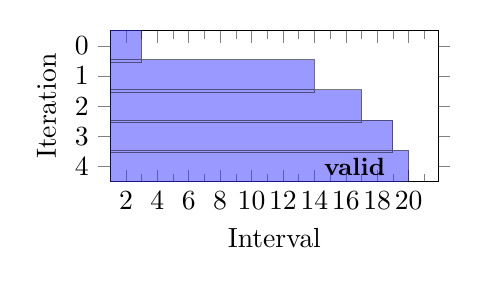
\begin{tikzpicture}
    \begin{axis}[
        xbar,
        xmin=1,
        width=5.75cm,
        height=3.5cm,
        xlabel={Interval},
        ylabel={Iteration},
        ytick=data,
        xtick distance=2,
        minor x tick num=1,
        x tick label as interval=false,
        y dir=reverse,
        ymin=-0.5,
        ymax=4.5,
        bar width=1.18em,
    ]
    \addplot+[black,fill=blue!80!white,opacity=0.5] coordinates {(20,4) (19,3) (17,2) (14,1) (3,0)};
    \node[
        anchor=west,
        font=\small,
    ] at (axis cs:14,4) {\textbf{valid}};
    \end{axis}
    \end{tikzpicture}
    \caption{Interval extension for \cref{eqn:max-return-to-resting-mtl}.}
    \label{fig:iterative-interval-extension}
\end{subfigure}%
\begin{subfigure}[t]{0.5\textwidth}
    \centering
    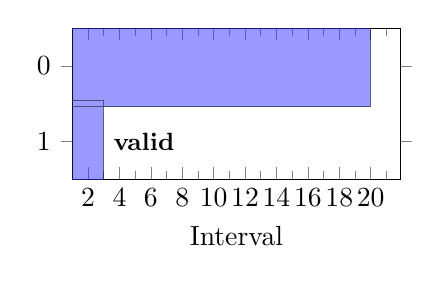
\begin{tikzpicture}
    \begin{axis}[
        xbar=1em,
        xmin=1,
        width=5.75cm,
        height=3.5cm,
        xlabel={Interval},
        ytick=data,
        xtick distance=2,
        minor x tick num=1,
        x tick label as interval=false,
        y dir=reverse,
        ymin=-0.5,
        ymax=1.5,
        bar width=2.95em,
    ]
    \addplot+[black,fill=blue!80!white,opacity=0.5] coordinates {(20,0) (3,1)};
    \node[
        anchor=west,
        font=\small,
    ] at (axis cs:3,1) {\textbf{valid}};
    \end{axis}
    \end{tikzpicture}
    \caption{Interval contraction for \cref{eqn:min-return-to-resting}.}
    \label{fig:iterative-interval-contraction}
\end{subfigure}
\caption{Iterative interval weakening to generate optimal, valid intervals.}
\end{figure}
%
We check our desired property (\cref{eqn:max-return-to-resting-mtl}) against our amended model, and can see in \cref{fig:iterative-interval-extension} that in four iterations of \cegiw{} we extended the interval, and ended with the optimal interval which was then verified to hold in the system. So, the optimal property that holds in our amended system is
\begin{equation}\label{eqn:max-return-to-resting-corrected}
    \mathcal{M}\vDash\Box(\texttt{resting} \rightarrow \eventually{[1,20]}\texttt{resting}).
\end{equation}
%
Another property we are interested in is not the maximum time that the robot can spend away from home, but the \emph{minimum}. We wish the robot to spend at least 20 time units away from home, formalised as
%
\begin{equation}\label{eqn:min-return-to-resting}
\mathcal{M}\vDash\Box((\texttt{resting}\land\eventually{[1,1]}\neg\texttt{resting}) \rightarrow \generally{[1,20]}\neg\texttt{resting}).
\end{equation}
%
Again, we check this against our modified model and can see in \cref{fig:iterative-interval-contraction} that it took only one iteration to contract the interval, reaching the optimal interval which was then verified to hold in the system as
%
\begin{equation}\label{eqn:min-return-to-resting-corrected}
\mathcal{M}\vDash\Box((\texttt{resting}\land\eventually{[1,1]}\neg\texttt{resting}) \rightarrow \generally{[1,3]}\neg\texttt{resting}).
\end{equation}
%
By using \cegiw{}, we first identified that the original specification had a design flaw that allowed unwanted infinite loops. After modifying the specification, we then deduced both the maximum time that the robot can stay away from home, as well as the minimum time.


\subsection{Applicability of Interval Weakening to Real-World Requirements (RQ2)}\label{subsec:case-studies}
%
\begin{table}[t]
\caption{Interval-weakenable requirements in \fret{} case studies.}
\label{table:weakenable-reqs-case-studies}
\centering
\begin{tabular}{ |l|r|r| } 
\hline
\textbf{Case study} & \textbf{Total requirements} & \textbf{Weakenable requirements} \\\hline
Mechanical lung ventilator~\cite{farrell2024} & 121 & 57 \\\hline
Autonomous drone~\cite{sheridan2025} & 62 & 19 \\\hline
Lift-plus-cruise aircraft~\cite{pressburger2023} & 49 & 29 \\\hline
Aircraft engine controller~\cite{farrell2022} & 42 & 0 \\\hline
Inspection rover~\cite{bourbouh2021} & 15 & 1 \\\hline
Grasping for debris removal~\cite{farrell2022a} & 20 & 0 \\\hline
Robotic patterns~\cite{vazquez2024} & 36 & 11 \\\hline
LMCP challenges~\cite{mavridou2020} & 74 & 7 \\\hline
\textbf{Total} & \textbf{419} & \textbf{124} \\\hline
\end{tabular}
\end{table}
%
\begin{figure*}[t]
    \centering
    \begin{subfigure}[t]{0.475\textwidth}
        \texttt{\textcolor{fret_condition}{upon ControlLoopStart}
        \textcolor{fret_component}{System}
        \textcolor{fret_shall}{shall}
        \textcolor{fret_timing}{within 12 milliseconds}
        \textcolor{fret_response}{satisfy ControlLoopFinish}}
        \caption{Autonomous drone requirement REQ018 describing the maximum time the control loop can take to complete.}
        \label{fig:example-fret-requirement-REQ018}
    \end{subfigure}%
    \hspace{1em}%
    \begin{subfigure}[t]{0.475\textwidth}
        \texttt{\textcolor{fret_condition}{if powerFailure}
        \textcolor{fret_component}{System}
        \textcolor{fret_shall}{shall}
        \textcolor{fret_timing}{for 120 minutes}
        \textcolor{fret_response}{satisfy !off}}
        \vspace{\baselineskip}
        \caption{Mechanical lung ventilator requirement FUN37 describing how long the system must stay on after power failure.}
        \label{fig:example-fret-requirement-FUN37}
    \end{subfigure}%
    \caption{Example \fretish{} requirements from the case studies. Both are taken from systems that are fully implemented and operational in real-world settings.}
\end{figure*}
%
In this section, we analyse existing requirements from a number of real-world case studies to assess how often interval weakening is applicable, and how weakened timing bounds can be interpreted in their respective domains. These requirements are formalised using the Formal Requirements Elicitation Tool (\fret{})~\cite{giannakopoulou2020a} and are written in \fretish{}, a structured natural language that can be translated to \MTL{}~\cite{giannakopoulou2021}. \fretish{} requirements can have a \texttt{\textcolor{fret_timing}{timing}} field, on which we can use interval weakening to weaken the requirement itself. The number of requirements that can be weakened using interval weakening per case study is shown in \cref{table:weakenable-reqs-case-studies}. As an example, the requirement in \cref{fig:example-fret-requirement-REQ018} from the autonomous drone case study~\cite{sheridan2025} uses the \texttt{\textcolor{fret_timing}{within 12 milliseconds}} timing which specifies that if the condition holds in one state, then the consequent must hold within the next twelve states (assuming that state transitions correspond to a millisecond of time passing). The \MTL{} translation of this timing corresponds to the \MTL{} temporal operator $\Diamond_{[0,12]}$, and so the requirement corresponds to
%
% We analyse the requirement sets from a number of case studies, which are formalised using the Formal Requirements Elicitation Tool (\fret{})~\cite{giannakopoulou2020a}. Requirements are written in \fretish{}, a structured natural language that can be translated to \MTL{}~\cite{giannakopoulou2021}. \fretish{} requirements can have a \texttt{\textcolor{fret_timing}{timing}} field, on which we can use interval weakening to weaken the requirement itself. The number of requirements that can be weakened using interval weakening per case study is shown in \cref{table:weakenable-reqs-case-studies}. As an example, the requirement in \cref{fig:example-fret-requirement-REQ018} from the autonomous drone case study~\cite{sheridan2025} uses the \texttt{\textcolor{fret_timing}{within 12 milliseconds}} timing which specifies that if the condition holds in one state, then the consequent must hold within the next twelve states (assuming that state transitions correspond to a millisecond of time passing). The \MTL{} translation of this timing corresponds to the \MTL{} temporal operator $\Diamond_{[0,12]}$, and so the requirement corresponds to
%
\begin{equation}\label{eqn:example-fret-requirement-REQ018}
\Box(\texttt{\textcolor{fret_condition}{ControlLoopStart}}\rightarrow \eventually{[0,12]}(\texttt{\textcolor{fret_response}{ControlLoopFinish}})).
\end{equation}
%
Under system degradation, for example if the onboard communications network is degraded so that commands take longer to reach control surfaces, we may not be able to guarantee this and so would have to weaken the property by extending the interval, giving more time for the system to run its control loop, with an example weakening in
%
\begin{equation}\label{eqn:example-fret-requirement-REQ018-weakened}
\Box(\texttt{\textcolor{fret_condition}{ControlLoopStart}}\rightarrow \eventually{[0,24]}(\texttt{\textcolor{fret_response}{ControlLoopFinish}})).
\end{equation}
%
An example requirement from the mechanical lung ventilator case study~\cite{farrell2024} is shown in \cref{fig:example-fret-requirement-FUN37}, and as the \fretish{} timing \texttt{\textcolor{fret_timing}{for 120 minutes}} corresponds to the \MTL{} temporal operator $\Box_{[1,120]}$, the corresponding \MTL{} property is
%
\begin{equation}\label{eqn:example-fret-requirement-FUN37}
\Box(\texttt{\textcolor{fret_condition}{powerFailure}} \rightarrow  \generally{[1,120]}(\neg\texttt{\textcolor{fret_response}{off}})).
\end{equation}
%
This is a regulatory requirement~\cite{iso2023} and so, if it does not hold in the degraded system, it is critical to know by exactly how much it is violated. We may only be able to guarantee that the ventilator will stay on for at most 90 minutes after \texttt{\textcolor{fret_condition}{powerFailure}}, producing the weakening
%
\begin{equation}\label{eqn:example-fret-requirement-FUN37-weakened}
\Box(\texttt{\textcolor{fret_condition}{powerFailure}} \rightarrow  \generally{[1,90]}(\neg\texttt{\textcolor{fret_response}{off}})).
\end{equation}
%
Of the 127 interval-weakenable requirements in \cref{table:weakenable-reqs-case-studies}, 116 can be weakened by interval extension as in \cref{eqn:example-fret-requirement-REQ018-weakened}, and 11 by interval contraction as in \cref{eqn:example-fret-requirement-FUN37-weakened}.

Several case studies in \cref{table:weakenable-reqs-case-studies} have few or no requirements that can be weakened with interval weakening. These requirements are typically liveness properties specified with the \texttt{\textcolor{fret_timing}{eventually}} timing, which cannot be weakened further, or safety properties specified with the \texttt{\textcolor{fret_timing}{always}} timing, for which interval weakening would not be appropriate. For example, from the grasping for debris removal case study~\cite{farrell2022a},
%
\begin{equation}\label{eqn:example-fret-requirement-always}
\texttt{\textcolor{fret_component}{SV}
\textcolor{fret_shall}{shall}
\textcolor{fret_timing}{always}
\textcolor{fret_response}{satisfy !collide(SV, TGT)}}.
\end{equation}
%
To answer \textbf{RQ2}, we have shown that interval weakening is applicable to a substantial proportion of existing temporal requirements, and that such weakenings have meaningful interpretations in safety-critical domains. We have also answered \textbf{RQ1} by using \cegiw{} to identify problems in a specification, and then deduce useful timing properties in the fixed system.

